\chapter{Lasso i lineære modeller}
\textit{I dette kapital introduceres lasso estimatoren for lineær regression. 
Først beskrives standard lasso og dens relation til ridge regression, hvorefter vi skitser en simple udregning af lasso.
Til slut introduceres teori for entydighed og konsistens af lasso estimatoren.} \\[4mm]
%
Givet \(n\) observationer betragtes responsvariablen \(y_i\) og en \(p \times 1\) vektor af forklarende variable eller prædiktorer \(\tx_i\), hvor \(j\)'te element betegnes \(x_{ij}\).
%Betragt \(n\) observationer \(\{\tx_i, y_i\}_{i=1}^n \), hvor $\tx_i=(x_{i1}, \ldots, x_{ip})$ er en $p$ dimensional vektor af forklarende variable eller prædiktorer og $y_i \in \R$ er den tilhørende responsvariabel.

Den velkendte estimator for mindste kvadraters metode (OLS) findes ved at minimere summen af kvadrerede residualer (SSR)
\begin{align}
\argmin_{\beta_0, \tbeta} \cbr{\sum_{i=1}^n \del{y_i - \beta_0 - \sum_{j=1}^p x_{ij} \beta_j}^2}. \label{eq:OLS}
\end{align}
%
Ofte standardiseres prædiktorerne, således at de er centreret \( \del{\frac{1}{n} \sum_{i=1}^n x_{ij} = 0}\) og har unit varians \( \del{\frac{1}{n} \sum_{i=1}^n x_{ij}^2=1}\).
Hvis ikke prædiktorerne standardiseres, da vil estimaterne afhænge af enhederne, som prædiktorerne er målt i.
For fuldstændighed centreres responsvariablen også \( \del{\frac{1}{n} \sum_{i=1}^n y_{i} = 0} \).
Hermed kan vi se bort fra skæringen $\beta_0$ i det givne optimeringsproblem.
Givet en optimal løsning \(\widehat{\tbeta}\) på det centreret data, kan vi finde løsningen for det ikke-centreret data: der gælder, at \(\widehat{\tbeta}\) er den samme og 
\(\widehat{\beta}_0 = \bar{y} - \sum_{j=1}^p \bar{x}_j \widehat{\beta}_j\), hvor \(\bar{y}\) og \(\bar{x}_j \) for \(j=1, \ldots, p\) er gennemsnittene for det ikke-centreret data.
Derfor ser vi bort fra skæringen i resten af dette kapitel samt kapitel \ref{ch:generalisering_lasso}, hvor generaliseringer af lasso estimatoren introduceres.

Lad \(\y\) være en \(n \times 1\) vektor med responsvariable og lad \(\X\) være en $n \times p$ matrix med  i'te række $\tx_i$, da kan \eqref{eq:OLS} omskrives til matrix-vektor form
\begin{align*}
\argmin_{ \tbeta} \cbr{ \Vert \y - \X \tbeta \Vert_2^2},
\end{align*}
hvor \(\Vert \cdot \Vert_2\) betegner den Euklidiske norm.
Som bekendt er løsningen hertil givet ved
\begin{align*}
\widehat{\tbeta}^{\text{OLS}} = (\X^T \X)^{-1} \X^T \y.
\end{align*}
OLS estimatoren er unbiased, men har ofte høj varians. 
Prædiktionen af responsvariablen kan ofte forbedres, hvis koefficienterne mindskes eller sættes direkte lig 0.
Dette vil give estimatoren lidt bias, men reducere variansen, hvilket forbedrer bias-variance tradeoff og dermed også prædiktionen.
En anden årsag til, at vi leder efter alternativer til OLS er, at med et højt antal prædiktorer ønsker vi, at bestemme en mindre delmængde af disse, som siger mest om responsvariablen, dvs forbedre fortolkningen.

Hvis \(p > n\), da kan \(\X\) ikke have fuld rang.
Det betyder, at $\X^T \X$ er singulær, og der findes derfor ikke en entydig estimator for OLS.

Nedenfor introduceres \textit{lasso estimatoren}, som kombinerer objektfunktionen i \eqref{eq:OLS} med en $\ell_1$-norm betingelse eller øvre grænse for summen af de absolutte værdier af koefficienterne.
Denne betingelse mindsker koefficienterne og sætter endda nogle lig 0. 
Dermed udfører metoden modeludvælgelse i lineær regression.
Det resulterende optimeringsproblem er konveks, og kan løses effektivt som beskrives nærmere i kapitel \ref{kap:optimeringsmetoder}.
%
\section{Lasso estimatoren} \label{sec:lasso_estimatoren}
\textit{Dette afsnit er skrevet udfra kapitel 2 i \citep{hastie}.}

\textit{The Least Absolute Shrinkage Selection Operator}, som forkortes lasso, blev introduceret af \citep{lasso}. 
Lasso finder løsningen til optimeringsproblemet
\begin{align}
\arg \min_{\beta} \cbr{\frac{1}{2n} \sum_{i=1}^n \del{y_i - \sum_{j=1}^p x_{ij} \beta_j}^2}, \ \text{underlagt at } \sum_{j=1}^p \vert \beta_j \vert \leq t, \label{eq:2.3}
\end{align} 
hvor vi bemærker, at betingelsen $\sum_{j=1}^p \vert \beta_j \vert \leq t$ kan skrives mere kompakt som en \(\ell_1\)-norm betingelse $\Vert \beta \Vert_1 \leq t$.

%På matrix-vektor form omskrives \eqref{eq:2.3} til
%\begin{align*}
%\arg \min_{ \beta} \cbr{\frac{1}{2n} \Vert \y - \X \beta \Vert_2^2}, \ \text{underlagt at } \Vert \beta \Vert_1 \leq t,
%\end{align*}
%hvor \(\Vert \cdot \Vert_2\) betegner den Euklidiske norm.
Værdi af \(t\) begrænser summen af de absolutte værdier af parameter estimaterne.
Den kontrollerer kompleksiteten af modellen. 
Større værdi af \(t\) betyder flere parametre og tillader dermed at modellen tilpasser data meget præcis.
Mindre værdi af \(t\) vil begrænse antallet af parametre, hvilket fører til mere sparse modeller, som tilpasser data mindre præcis.
Værdien af \(t\) skal specificeres ved en ekstern procedure kaldet \textit{krydsvalidering}, som vil blive diskuteret i kapitel \ref{kap:statistisk_inferens}.

Lasso problemet kan omskrives til Lagrange form
\begin{align}
\hat{\beta}^\text{lasso} = \arg \min_{\beta} \cbr{\frac{1}{2n} \Vert \y - \X \beta \Vert_2^2 + \lambda \Vert \beta \Vert_1}, \label{eq:2.5}
\end{align}
hvor $\lambda \geq 0$ er en såkaldt strafparameter, som også bestemmes udfra krydsvalidering. 
Der er en en-til-en korrespondance mellem det betingede problem \eqref{eq:2.3} og Lagrange problemet \eqref{eq:2.5}. 
For hver værdi af \(t\) hvor \(\Vert \beta \Vert_1 \leq t\) er opfyldt, da findes en tilhørende værdi af $\lambda$ som giver den samme løsning for \eqref{eq:2.5}.
Omvendt gælder der, at løsningen $\hat{\beta}_\lambda$ til \eqref{eq:2.5} løser grænse problemet med $t=\Vert \hat{\beta}_\lambda \Vert_1$.

I andre beskrivelser af lasso estimatoren ses det at faktoren \(\frac{1}{2n}\) i \eqref{eq:2.3} og \eqref{eq:2.5} erstattes med \(\frac{1}{2}\) eller \(1\).
Dette gør ingen forskel i \eqref{eq:2.3} og svarer blot til en simpel reparametrisering af \(\lambda\) i \eqref{eq:2.5}.
Denne standardisering gør \(\lambda\) værdierne sammenlignelige for samples size af forskellige størrelse, som er brugbart i krydsvalidering.

\textit{Ridge regression} estimatoren findes udfra 
\begin{align} 
\hat{\beta}^\text{ridge} = \arg \min_{\beta} \cbr{\frac{1}{2n} \sum_{i=1}^n \del{y_i - \sum_{j=1}^p x_{ij} \beta_j}^2}, \ \text{underlagt at } \sum_{j=1}^p \beta_j^2 \leq t, \label{eq:2.7} 
\end{align} 
%som kan omskrives på Lagrange form
%\begin{align} 
%\arg \min_{\beta} \cbr{\frac{1}{2n} \sum_{i=1}^n \del{y_i - \sum_{j=1}^p x_{ij} \beta_j}^2 + \lambda \sum_{j=1}^p \beta_j^2}, 
%\end{align} \label{eq:2.8} 
%hvor $\lambda \geq 0$.
som kan omskrives på Lagrange form
\begin{align*}
\hat{\beta}^\text{ridge} = \arg \min_{\beta} \cbr{\frac{1}{2n} \Vert \y - \X \beta \Vert_2^2 + \lambda \Vert \beta \Vert_2^2},
\end{align*}
hvor $\lambda \geq 0$.
Heraf kan ridge regression estimatoren findes ved at differentiere \(\del{\y - \X \beta}^T \del{\y - \X \beta} + \lambda \beta^T \beta\) mht $\beta$, sætte dette lig 0 og isolere for $\beta$. Hvoraf vi finder, at
\begin{align*} 
\hat{\beta}^\text{ridge} = (\X^T \X + \lambda I_p)^{-1} \X^T \y. 
\end{align*}  
I forhold til mindste kvadraters regression tilføjer ridge regression en positiv konstant $\lambda$ på diagonalen af $\X^T \X$, hvilket medfører, at \(\X^T \X\) er invertibel, selvom $\X$ ikke har fuld rang. 
Dermed er en entydig løsning altid garanteret. 

Lad os betragte data givet i tabel \ref{tab:crime}.
For 50 byer i United States er kriminalitetsraten per 1 million indbyggere givet og følgende 5 prædiktorer: 
\begin{itemize}
\item \texttt{funding}: årlige politiske finansiering i dollars per indbygger
\item \texttt{hs}: procentvise andel af 25 årige eller derover med 4 års gymnasial uddannelse
\item \texttt{not-hs}: procentvise andel af 16-19 årige som ikke går i gymnasiet og ikke har en gymnasiel uddannelse
\item \texttt{college}: procentvise andel af 18-24 årige som studerer på universitetet
\item \texttt{college4}: procentvise andel af 25 årige eller derover med mindst 4 år på universitetet
\end{itemize}
%
\begin{table}[ht] 
\centering 
\begin{tabular}{c|cccccc} 
\texttt{city} & \texttt{funding} & \texttt{hs} & \texttt{not-hs} & \texttt{college} & \texttt{college4} & \texttt{crime rate} \\
\midrule
1 & 40 & 74 & 11 & 31 & 20 & 478 \\
2 & 32 & 72 & 11 & 43 & 18 & 494 \\
3 & 57 & 70 & 18 & 16 & 16 & 643 \\
4 & 31 & 71 & 11 & 25 & 19 & 341 \\
5 & 67 & 72 & 9 & 29 & 24 & 773 \\
\vdots & \vdots & \vdots & \vdots & \vdots & \vdots & \vdots \\
50 & 66 & 67 & 26 & 18 & 16 & 940 \\
\bottomrule
\end{tabular}  
\caption{Kriminalitetsraten og fem prediktorer for \(n=50\) stater i United States.} \label{tab:crime} 
\end{table} 
%
Datasættet, som vi betegner crime data, er inkluderet for at underbygge teorien og vi vil løbende i rapporten referere til det.
På figur \ref{fig:crime_koef} anvendes crime data til at illustrere koefficientstierne for henholdsvis ridge regression og lasso.
%
\begin{figure}[H]
\centering
\begin{minipage}{0.4\linewidth}
\scalebox{0.32}{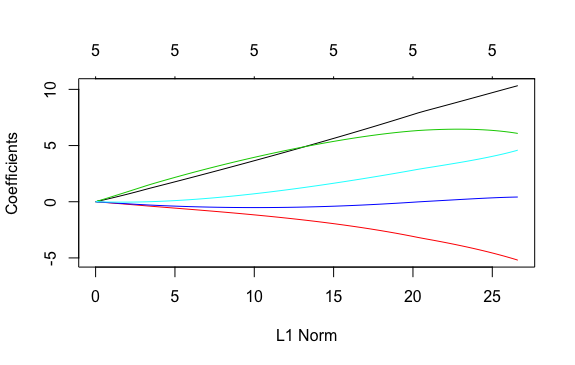
\includegraphics{fig/crime_ridge.png}}
\end{minipage}
\hspace{0.2cm}
\begin{minipage}{0.4\linewidth}
\scalebox{0.32}{\includegraphics{fig/crime_lasso.png}}
\end{minipage}
\caption{Koefficientstierne for ridge regression (venstre) og lasso (højre) plottet imod \(\ell_1\)-normen.} \label{fig:crime_koef}
\end{figure}

Variabel udvægelsen for ridge regression og lasso illustreres på figur \ref{fig:LassoRig}.
\begin{figure}[H]
\centering
\begin{minipage}{0.4\linewidth}
\scalebox{0.7}{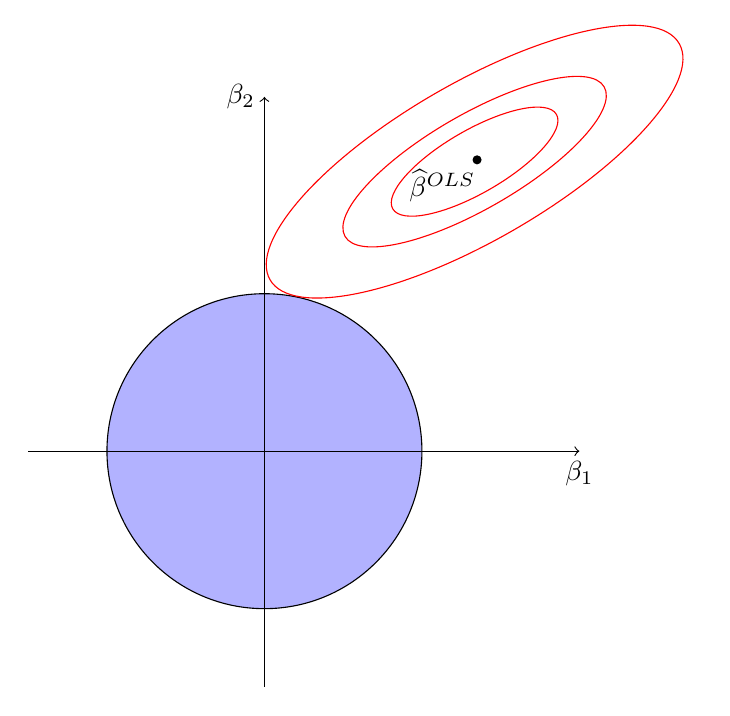
\begin{tikzpicture}
\draw [fill] (2.7,3.7) circle [radius=0.05];
\node [below left] (a) at (2.8,3.7) {$\widehat{\boldsymbol{\beta}}^\text{OLS}$};
\draw (0,0) circle (2cm) [fill= blue!30];
\draw [<-] (0,4.5) node [left] {$\beta_2$}-- (0,-3);
\draw[<-] (4,0) node [below] {$\beta_1$} -- (-3,0);
\begin{scope}[rotate = 30, red]
\clip[draw] (4.15,1.85) ellipse (3cm and 1cm);
\clip[draw] (4.15,1.85)ellipse (1.9 cm and 0.6 cm); 
\clip[draw] (4.15,1.85) ellipse (1.2 cm and 0.4 cm);
\end{scope}
\end{tikzpicture}}
\end{minipage}
\hspace{0.2cm}
\begin{minipage}{0.4\linewidth}
\scalebox{0.7}{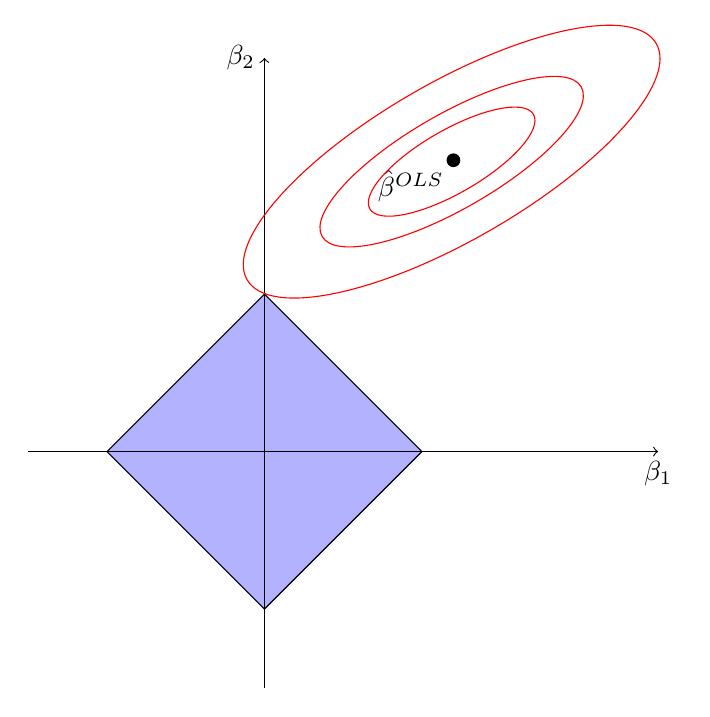
\begin{tikzpicture}
\draw [fill] (2.4,3.7) circle [radius=0.08];
\node [below left] (a) at (2.4,3.7) {$\hat{\beta}^\text{OLS}$};
\draw (-2,0) -- (0,2) -- (2,0)-- (0,-2) -- (-2,0)[fill = blue!30];
\draw [<-] (0,5) node [left] {$\beta_2$}-- (0,-3);
\draw[<-] (5,0) node [below] {$\beta_1$} -- (-3,0);
\begin{scope}[rotate = 30, red]
\clip[draw] (3.9,2) ellipse (3cm and 1cm);
\clip[draw] (3.9,2)ellipse (1.9 cm and 0.6 cm); 
\clip[draw] (3.9,2) ellipse (1.2 cm and 0.4 cm);
\end{scope}
\end{tikzpicture}}
\end{minipage}
\caption{Konturer for SSR og betingelsesområderne for ridge regression (venstre) og lasso (højre). De blå arealer er betingelsesområderne $\vert \beta_1 \vert+\vert \beta_2 \vert \leq t$ og $\beta_1^2+\beta_2^2 \leq t^2$, mens de røde ellipser er konturkurver for SSR. Konturkurverne har centrum i OLS estimatoren, $\hat{\beta}^\text{OLS}$.} \label{fig:LassoRig}
\end{figure}
For $p=2$ underligges OLS betingelsen $\beta_1^2 + \beta_2^2 \leq t^2$ for ridge regression og betingelsen $\vert \beta_1 \vert + \vert \beta_2 \vert \leq t$ for lasso.
Ellipserne omkring $\hat{\beta}^{\text{OLS}}$ er konturkurverne for SSR, dvs. SSR er konstant i en given ellipse. Værdien af SSR stiger, som ellipsen udvides fra $\hat{\beta}^{\text{OLS}}$.
Løsningen for ridge regression og lasso er givet ved det første punkt, hvor konturkurverne rammer betingelsesområderne.
Da ridge regression har et cirkulært betingelsesområde, vil skæringen med konturkurverne generelt ikke forekomme direkte på en akse.
Omvendt har lasso et regulært betingelsesområde med hjørner i hver akse, hvilket betyder, at hvis løsningen forekommer i et hjørne, da vil en af parametrene $\beta_j$ være lig 0.

Hvis $t$ er tilstrækkelig stor, da vil betingelsesområderne indeholde $\hat{\beta}^{\text{OLS}}$ og derfor vil ridge regression og lasso estimatorerne være lig OLS estimatoren.

På figur \ref{fig:LassoRig} har vi blot betragtet det simple tilfælde hvor $p=2$. Når $p=3$ vil betingelsesområdet for ridge regression være en kugle, mens betingelsesområdet for lasso vil være en polydron. 

\begin{lem}
Givet data \(\del{\y, \X}\), defineres et augmented datasæt
\begin{align*}
\mathbf{X}^* = \begin{bmatrix}
\mathbf{X} \\ \sqrt{\lambda} I_p
\end{bmatrix}, \quad 
\mathbf{y}^* = \begin{bmatrix}
\mathbf{y} \\ 0_p
\end{bmatrix},
\end{align*}
hvor \(\X^* \in \mathbb{R}^{\del{n+p} \times p}\) og \(\y^* \in \mathbb{R}^{n+p}\). Da kan estimatoren for ridge regression udledes udfra mindste kvadraters metode.
\end{lem}
\begin{proof}
Vi har, at
\begin{align*}
\del{\X^{*^T} \X^*}^{-1} \X^{*^T} \y^* &= \left( \begin{bmatrix}
\mathbf{X} & \sqrt{\lambda} I_p
\end{bmatrix}
\begin{bmatrix}
\mathbf{X} \\ \sqrt{\lambda} I_p
\end{bmatrix} \right)^{-1}
\begin{bmatrix}
\mathbf{X} & \sqrt{\lambda} I_p
\end{bmatrix}
\begin{bmatrix}
\mathbf{y} \\ 0
\end{bmatrix} \\
&= \left( \mathbf{X}^T \mathbf{X} + \lambda I_p \right)^{-1} \mathbf{X}^T \mathbf{y}.
\end{align*}
\end{proof}


\subsection{Udregning af lasso}
Da lasso strafleddet ikke er differentialbel, findes der ikke en eksplicit løsning til optimeringsproblemet for lasso.
En simpel procedure kaldet \textit{coordinate descent} kan udfra lagrange formen udregne en numerisk løsning. 

\subsubsection{Single prædiktor: soft tresholding}
Vi betragter blot en enkelt prædiktor \(z_i\). 
Problemet, som vi skal løse, er da
\begin{align*}
\arg \min_{\beta} \cbr{\frac{1}{2n} \sum_{i=1}^n \del{y_i - z_{i} \beta}^2 + \lambda \vert \beta \vert}.
\end{align*}
Som bekendt er standard proceduren at finde den første ordens afledede mht $\beta$, sætte denne lig 0 og isolere for $\beta$. 
Men vi bemærker, at \(\vert \beta \vert \) ikke har en afledt i $\beta=0$.
Vi kan dog fortsætte ...
Vi finder, at
\begin{align*}
\frac{\partial}{\partial \beta} \del{\frac{1}{2n} \sum_{i=1}^n \del{y_i - z_{i} \beta}^2 + \lambda \vert \beta \vert}
&= -\frac{1}{n} \sum_{i=1}^n \del{y_i - z_{i} \beta} z_i + \begin{cases}
-\lambda \quad &\beta < 0 \\
[-\lambda, \lambda] & \beta = 0 \\
\lambda & \beta >0 
\end{cases}  \\
&= -\frac{1}{n} \left\langle \mathbf{z}, \mathbf{y} \right\rangle + \beta + \begin{cases}
-\lambda \quad &\beta < 0 \\
[-\lambda, \lambda] & \beta = 0 \\
\lambda & \beta >0 
\end{cases},
\end{align*}
da $\frac{1}{n} \sum_{i=1}^n z_i^2=1$. Dette sættes lig 0 og vi isolerer $\beta$, hvoraf vi finder, at
\begin{align}
\hat{\beta} = \begin{cases}
\frac{1}{n} \left\langle \mathbf{z}, \mathbf{y} \right\rangle - \lambda, \quad &\frac{1}{n} \left\langle \mathbf{z}, \mathbf{y} \right\rangle > \lambda, \\
0 &\frac{1}{n} \left\langle \mathbf{z}, \mathbf{y} \right\rangle \leq \lambda, \\
\frac{1}{n} \left\langle \mathbf{z}, \mathbf{y} \right\rangle + \lambda, &\frac{1}{n} \left\langle \mathbf{z}, \mathbf{y} \right\rangle < \lambda.
\end{cases} \label{eq:2.10}
\end{align}
Definer \textit{soft-threshold operatoren}
\begin{align*}
S_\lambda\del{x}=\text{sign}\del{x} \del{\vert x \vert - \lambda}_+,
\end{align*}
som trækker argumentet $x$ mod 0 med $\lambda$, og sætter den lig med 0 hvis $\vert x \vert \leq \lambda$. 
Figur \ref{fig:soft_thresholding_fct} illustrerer operatoren.
Da kan vi omskrive \eqref{eq:2.10} til
\begin{align*}
\hat{\beta} = S_\lambda \del{\frac{1}{n} \left\langle \mathbf{z}, \mathbf{y} \right\rangle}.
\end{align*}
%
\begin{figure}[H]
\centering
\scalebox{0.8}{\begin{tikzpicture}
\draw (-2.5,-2.5) -- (2.5,2.5);
\draw[dashed] (-2.5,-1.7) -- (-0.75,0) -- (0.75,0) -- (2.5,1.7); 
\draw[dotted] (2.5,1.7) -- (2.5,2.5);
%\draw node [label={[xshift=0.5cm, yshift=-0.8cm]$\del{0,0}$}] {};
\draw node [label={[xshift=2.75cm, yshift=1.8cm]$\lambda$}] {};
\draw [<-] (0,3) node [left] {$S_\lambda \del{x}$}-- (0,-3);
\draw[<-] (3,0) node [below] {$x$} -- (-3,0);
\end{tikzpicture}}
\caption[optional short text]{Soft thresholding funktionen $S_\lambda\del{x}=\text{sign}\del{x} \del{\vert x \vert - \lambda}_+$.} \label{fig:soft_thresholding_fct}
\end{figure}
%
\subsubsection{Multiple prædiktorer: cyclic coordinate descent}
Herefter kan vi betragte multivariate prædiktorer. 
%Gentagne cycle gennem prædiktorerne i en fast, men vilkårlig orden $j=1, 2, \ldots, p$, hvor koefficienten $\beta_j$ opdateres i det $j$'te step, ved at minimere objektfunktionen i dens koordinat, mens de resterende koefficienter $\cbr{\hat{\beta}_k, k \neq j}$ fastholdes deres nuværende værdier. 
Vi kan opskrive objektfunktionen i \eqref{eq:2.5} som
\begin{align*}
\frac{1}{2n} \sum_{i=1}^n \del{y_i - \sum_{k \neq j} x_{ik} \beta_k - x_{ij} \beta_j}^2 + \lambda \sum_{j = 1}^p \vert \beta_j \vert
\end{align*}
Definer den partialle residual $r_i^{(j)}=y_i - \sum_{k \neq j} x_{ik} \hat{\beta}_k$, som fjerner nuværende fit fra den $j$'te prædiktor.
Da er den j'te koefficient opdateret ved
\begin{align}
\hat{\beta}_j = S_\lambda \del{\frac{1}{n} \left\langle \mathbf{x}_j, \mathbf{r}^{(j)} \right\rangle}, \label{eq:2.14}
\end{align}
hvor \(r_i = y_i - \sum_{j = 1}^p x_{ij} \hat{\beta}_j \) er de fulde residualer.
Den beskrevne algoritme svarer til metoden \textit{cyclical coordinate descent}, som minimerer en konveks objektfunktion langs hver koordinat af gangen.
Under milde regularitetsbetingelser konvergerer løsningen til et global optimum.
Fra opdateringen \eqref{eq:2.14} ser vi, at algoritmen foretager en univariat regression af den partial residual på hver prædiktor, cycling gennem prædiktorerne indtil konvergens. \\

Ofte er vi interesseret i, at finde lasso løsningen for en mængde af \(\lambda\) værdier og ikke blot én fast lambda.
\textit{pathwise coordinate descent} kan anvendes hertil, ved at begynde med en værdi af \(\lambda\) som præcis er høj nok således at den optimale løsning er vektor bestående af \(0\).
Denne værdi er lig \(\lambda_{\max}=\max_j \vert \frac{1}{2} \left\langle \mathbf{x}_j, \y \right\rangle \vert\).
Da kan vi aftage \(\lambda\) med en lille mængde og køre coordinate descent undtil konvergens.
Aftage \(\lambda\) igen og anvende den tidligere løsning som en warm start, da kan vi kører coordinate descent indtil konvergens.
Hermed kan vi udregne løsningen over en grid af \(\lambda\) værdier. \\

Coordinate descent er særlig hurtig til at løse lasso problemet, da koordinatvis minimering er tilgængelig \eqref{eq:2.14}, og dermed er en iterativ søgning langs hver koordinat ikke nødvendig.
Derudover udnytter coordinat descent at lasso giver sparse løsninger.
For tilstrækkelige høje \(\lambda\) værdier er de fleste koefficienter lig $0$. \\[2mm] 
%
\textit{Homotopy metoder} er en alternativ teknisk til at løse lasso problemet. Disse producerer en helt sti af løsninger i en frekventiel sekvens, ved at starte med nul.
Denne sti er faktisk piecewise lineær.
Algoritmen kaldet \textit{least angle regression} (LARS) er en homotopy metode som effektivt konstruerer piecewise lineære stier.
En mere teoretisk gennemgang af coordinate descent og LARS algoritmen er givet i kapitel \ref{kap:optimeringsmetoder}. \\[2mm]


Hvis prædiktorerne er ortogonale, dvs $\frac{1}{n} \left\langle \mathbf{x}_j, \mathbf{x}_k \right\rangle = 0$ for alle $j \neq k$.
Da reduceres opdateringen \eqref{eq:2.14} til
\begin{align*}
\hat{\beta}_j = S_\lambda \del{\frac{1}{n} \left\langle \mathbf{x}_j, \mathbf{y} \right\rangle},
\end{align*}
dermed er $\hat{\beta}_j$ blot soft-thresholded version af det univariate mindste kvadraters estimat af $\mathbf{y}$ regresseret imod $\mathbf{x}_j$. Således har vi en lukket løsning og ingen iterationer er påkrævet.

\subsection{Frihedsgrader}
Antag at, vi har \(p\) prediktorer og tilpasser en lineær regressions model udfra \(k\) af disse prediktorer.
Hvis disse \(k\) prediktorer vælges uafhængigt af responsvariablen, da "anvender" fitting proceduren \(k\) frihedsgrader.
Dvs at teststørrelsen for at teste hypotesen om at alle \(k\) koefficienter er 0, har en Chi-squared fordeling med \(k\) frihedsgrader.

Hvis valget af de \(k\) prediktorer afhænger af responsvariablen, da forventes det at fitting proceduren anvender mere end \(k\) frihedsgrader. 
Vi kalder sådan en fitting procedure \textit{adaptiv}, og tydeligvis er lasso et eksempel på dette.

Ligeledes er forward-stepwise proceduren adaptiv, hvor vi sekventiel tilføjer prediktorer som mindsker fejlen mest.
Her forventes det at modellen anvender mere end \(k\) frihedsgrader efter \(k\) step.
Derfor er antallet af frihedsgrader ikke nødvendigvis lig med antallet af ikke-nul koefficienter.

Men for lasso er antallet af frihedsgrader faktisk lig antallet af ikke-nul koefficienter, som vi nu vil beskrive.

Først defineres hvad vi mener med frihedsgrader for en adaptiv fitted model. 
Antag at, vi har en additive-error model
\begin{align*}
y_i = f \del{x_i} + \epsilon_i, \quad i = 1, \ldots, n,
\end{align*}
hvor \(f\) er ukendt og \(\epsilon_i \sim iid \del{0, \sigma^2}\).
Lad \(\hat{\y}\) betegne \(n\) sample prediktorer, da defineres 
\begin{align*}
\text{df}\del{\hat{\y}} := \frac{1}{\sigma^2} \sum_{i=1}^n \text{Cov}\del{\hat{y}_i, y_i}.
\end{align*}
Antal frihedsgrader svarer da til indflydelsen hver respons mål har på dens prediktion.
Desto bedre modellen tilpasser data, desto højere antal frihedsgrader.
Det kan vises at, lasso med en fast strafparameter \(\lambda\) er antallet af ikke-nul koefficienter \(k_\lambda\) et unbiased estimat af frihedsgrader.

Som nævnt ovenfor anvender forward-stepwise regression mere end \(k\) frihedsgrader efter \(k\) step.
Lasso udvælger ikke blot prediktorer, som bekendt øger antallet af frihedsgrader, men shrinks også koefficienterne mod 0 relativ til mindste kvadraters estimaterne.
Denne skrinkage er netop tilstrækkelig til at brige antallet af frihedsgrader til \(k\).
Dette resultat er særligt nyttig, da det giver et kvalitativ mål af mængden af fitting som vi har opnået ved ethvert punkt på lasso stien.
Generelt er bevises for dette resultat meget besværligt.
Men i det ortogonale tilfælde ...

Ideen tages et skridt videre i sektion \ref{subsec:kovarians_test} hvor vi beskriver \textit{kovarians testen} til at teste significancen af prediktorerne ift lasso.


\subsubsection{Ikke-negative garrote}
\textit{Ikke-negative garrote}, introduceret af \citep{nonnegative_garrote}, er en two-stage procedure. 
Givet et initial estimat af regression koefficienterne \(\tilde{\beta} \in \mathbb{R}^p\), kan vi løse optimeringsproblemet
\begin{align}
\hat{\beta}_j^\text{garotte} = \arg \min_{c \in \mathbb{R}^p}  \cbr{ \sum_{i=1}^n \del{y_i - \sum_{j=1}^p c_j x_{ij} \tilde{\beta}_j}^2}, \ \text{underlagt at } c_j \geq 0 \text{ og } \Vert c \Vert_1 \leq t. \label{eq:2.19}
\end{align}
Lad \(\hat{\beta}_j^\text{garotte} = \hat{c}_j \cdot \tilde{\beta}_j\), for \(j = 1, \ldots, p\).
Der er en ækvivalent Lagrange form for denne procedure
\begin{align*}
\hat{\beta}_j^\text{garotte} = \arg \min_{c \in \mathbb{R}^p}  \cbr{\Vert \y - \X \beta \Vert_2^2 + \lambda \Vert c \Vert_1}, \ \text{underlagt at } c_j \geq 0.
\end{align*}
I den originale artikel \citep{nonnegative_garrote}, er initial estimatet \(\tilde{\beta}\) valgt til at være \(\hat{\beta}_j^\text{OLS}\)

Antag \(\X\) er ortogonal og \(t\) er således at betingelsen \(\Vert c \Vert_1 = t\) er opfyldt, da er
\begin{align*}
\hat{c}_j = \del{1 - \frac{\lambda}{\tilde{\beta}_j^2}}_+, \ j = 1, \ldots, p,
\end{align*}
hvor \(\lambda\) er valgt således at \(\Vert \hat{c} \Vert_1 = t\).
Hvis koefficienten \(\tilde{\beta}_j\) er stor, da vil shrinkage faktoren være tæt på 1, dvs ingen shrinkage, men hvis den er lille, da vil estimatet blive shrunkage mod 0.
Af figur \ref{fig:nonnegative_garrote} ses det, at garrote shrinker lave værdier af \(\beta\) hårdere end lasso, og omvendt for høje værdier.
%
\begin{figure}[H]
\centering
\scalebox{0.8}{\begin{tikzpicture}
%\draw[loosely dotted] (-3,-3) -- (3,3);
%\draw[dotted] (-3,-2) -- (3,2);
%\draw (-3,-1.5) -- (-0.75,0) -- (0.75,0) -- (3,1.5);
\draw (-3,-3) -- (3,3);
\draw[dashed] (-3,-2.2) -- (-0.75,0) -- (0.75,0) -- (3,2.2);
\draw[dotted] (-3,-2.6) -- (-1,0) -- (1,0) -- (3,2.6);
\draw [<-] (0,3.5) node [left] {$\hat{\beta}$}-- (0,-3.5);
\draw[<-] (3.5,0) node [below] {$\beta$} -- (-3.5,0);
\end{tikzpicture}}
\caption[optional short text]{Eksakte løsninger for lasso (\tikz[baseline]{\draw[dashed] (0,.5ex)--++(.5,0) ;}) og nonnegative garrote (\tikz[baseline]{\draw[dotted] (0,.5ex)--++(.5,0) ;}).} \label{fig:nonnegative_garrote}
\end{figure}
%
Nonnegaitve garrote er tæt relateret med adaptive lasso, som vi vil diskutere nærmere i afsnit ---.

-- viste at nonnegative garrote er path-konsistent under mindre strenge betingelser end lasso.
Dette gælder, hvis initial estimaterne er \(\sqrt{n}\)-konsistent, som inkluderer mindste kvadraters metoder (når \(p < n\)), lasso og elastisk net.
Path-konsistent betyder, at løsningsstien inkluderer den sande model.
Konvergens af parameter estimaterne for nonnegative garrote er langsommere end den af initial estimatet.
\newpage
 
\section{Entydighed af lasso estimatoren}
Løsningen til lasso problemet er entydig, hvis kolonnerne af \(\X\) er i general position (se definition \ref{defn:general_position}) jævnfør \citep{lasso_unique}.
Dette gælder også, når \(p \geq n\), selvom antallet af ikke-nul koefficienter er højst \(n\).
Hvis \(\X\) ikke har fuld rang, da er de fittede værdier entydige, mens parameter estimaterne ikke er.
Dette ikke-fuld rang tilfælde sker, når \(p \leq n\) grundet kollinaritet og sker altid når \(p>n\).
 


Derfor kan lasso kun være ikke-entydig for diskret data, som kommer af dummy-værdi kodning eller kategorisk prædiktorer.

Numeriske algoritmer for at løse lasso problemet vil typisk give gyldig løsninger i det ikke-entydige tilfælde.
Men løsningerne vil afhænge af algoritmen, f.eks. har valget af begyndelsesværdier indflydelse på den endelige løsning for coordinate descent.

%
%Lasso løsningen er entydige når \(\text{rank} \del{X}=p\), da lasso da er streng konveks.
%Men ikke streng konveks når \(\text{rank} \del{X} < p\) og der findes multiple minimizers af lasso problemet.
%Når antallet af variabler er større end antallet af observationer, \(p>n\), da må vi have at  \(\text{rank} \del{X} < p\).



\section{Konsistens af lasso estimatoren}
I dette afsnit ser vi nærmere på lasso estimatorens asymptotiske egenskaber.

For en estimator som udfører variabeludvælgelse, findes nogle såkaldte \textit{oracle egenskaber}.
En estimator som opfylder disse egenskaber, udvælger de sande kieffcienter!?! og de estimerede koefficienter følger asymptotisk en normal fordelingen.
Nedenfor defineres oracle egenskaberne.

\subsection{Orakelegenskaberne} 
Lad $\mathcal{A} =\{j:\beta_j^* \neq 0\}$, hvor $\beta_j^*$ betegner koefficienten af $x_j$ i den sande model og antag at $\vert \mathcal{A} \vert=p_0 <p$, således at den sande model afhænger af en delmængde af prædiktorerne. 
Så defineres orakelegenskaberne som følgende. 
\begin{defn}[Orakelegenskaber]
\begin{itemize}
\item Variabeludvælgelsen er konsistent, dvs for
\begin{align*}
\mathcal{A}_n=\lbrace j :\hat{\beta}_j \neq 0 \rbrace \ \text{og} \ \mathcal{A} =\{j:\beta_j^* \neq 0\},
\end{align*}
gælder der, at $\lim_{n \rightarrow \infty }P(\mathcal{A}_n=\mathcal{A})=1$.
\item Estimatoren er asymptotisk normalfordelt, dvs
\begin{align*}
\sqrt{n}(\hat{\boldsymbol{\beta}}_\mathcal{A}-\boldsymbol{\beta}^*_\mathcal{A}) \overset{d}{\rightarrow} N(\mathbf{0}, \boldsymbol{\Sigma}^*_I),
\end{align*}
hvor $\boldsymbol{\beta}^*_\mathcal{A}=\{ \beta_j^*, j \in \mathcal{A} \}$ og $\boldsymbol{\Sigma}^*_I$ er kovariansmatricen, hvor vi antager, at vi kender den sande model.
\end{itemize}
\end{defn}
Det er argumenteret for at en god procedure bør have disse orakel egenskaber.
Dog børe procedure have nogle ekstra betingelser udover orakel egenskaberne for at være optimal, såsom kontinuert shrinkage.
Derfor er det vigtigt at understrege at orakelegenskaber ikke alene resultere i en optimal prædiktion performance.

Lad os antage følgende
\begin{align*}
y_i = \x_i \beta^* + \epsilon_i, 
\end{align*}
hvor \(\epsilon_1, \ldots, \epsilon_n\)
Derudover antages det, at \(\frac{1}{n} \X^T \X \rightarrow \textbf{C}\), hvor
\begin{align*}
\textbf{C} = 
\begin{bmatrix}
\textbf{C}_{11}& \textbf{C}_{12}\\
\textbf{C}_{21}& \textbf{C}_{22}
\end{bmatrix},
\end{align*}
er en positiv definit matrix, hvor $\textbf{C}_{11}$ er en $p_0 \times p_0$ matrix. 
Lad os betragte lasso estimatet
\begin{align*}
\hat{\beta}^\text{lasso} = \argmin_\beta \Vert \y - \sum_{j=1}^p \x_j \beta_j \Vert_2^2 + \lambda_n \sum_{j=1}^p \vert \beta_j \vert,
\end{align*}
hvor \(\lambda_n\) varierer med \(n\).



%Så kan det udledes af proposition \ref{lem:lasso_consistency1}, at lasso ikke er konsistent i variabel udvælgelse i alle tilfælde og dermed ikke opfylder orakelegenskaberne.
%
\begin{lem}\label{lem:lasso_consistency1}
Hvis $\frac{\lambda_n}{\sqrt{n}} \rightarrow \lambda_0 \geq 0$, da vil $\hat{\beta}^\text{lasso} \overset{p}{\rightarrow} \argmin V_1$, hvor
\begin{align*}
V_1 \del{\mathbf{u}} = \del{\mathbf{u} - \beta^*}^T \mathbf{C} \del{\mathbf{u} - \beta^*} + \lambda_0 \sum_{j=1}^p \vert u_j \vert.
\end{align*}
\end{lem}
\begin{proof}
Beviset undlades, men der henvises til s. 1358 i \citep{adaptive_lasso_knight}.
\end{proof}
%
\begin{lem}\label{lem:lasso_consistency2}
Hvis $\frac{\lambda_n}{\sqrt{n}} \rightarrow \lambda_0 \geq 0$, da vil \(\sqrt{n} \del{\hat{\beta}^\text{lasso} - \beta^*} \overset{d}{\rightarrow} \argmin V_2\), hvor
\begin{align*}
V_2 \del{\mathbf{u}} = -2 \mathbf{u}^T \mathbf{W} + \mathbf{u}^T \mathbf{C} \mathbf{u} + \lambda_0 \sum_{j=1}^p \sbr{u_j \text{sign} \del{\beta^*_j} \mathbb{1} \del{\beta_j^* \neq 0} + \vert u_j \vert \mathbb{1} \del{\beta_j^* = 0}},
\end{align*}
og \(\mathbf{W} \sim N\del{\mathbf{0}, \sigma^2 \mathbf{C}}\).
\end{lem}
%
Af lemma \ref{lem:lasso_consistency2} har vi, at lasso estimatet er rod-n konsistent.

Hvis $\lambda_0=0$, da gælder ifølge lemma \ref{lem:lasso_consistency1}, at $\hat{\boldsymbol{\beta}}^\text{lasso} \overset{p}{\rightarrow} \hat{\boldsymbol{\beta}}^{*}$, da strafleddet forsvinder og $\mathbf{C}$ er en positiv definit matrix, og dermed er $\hat{\boldsymbol{\beta}}^\text{lasso}$ svagt konsistent. Men da strafleddet forsvinder, medfører det også, at lasso asymptotisk ingen variabeludvælgelse har. Hvis $\lambda_0>0$ kan det ikke udledes fra proposition \ref{prop:lasso_no_vs}, om estimatoren er konsistent. Det angives i \citep{adaptive_lasso}, at dette kun vil være tilfældet, når en given betingelse er opfyldt. En metode, der konsekvent udfører konsistent variabeludvælgelse, kan dog opnås med en simpel tilføjelse til lasso estimatet. Denne metode kaldes adaptive lasso.


%I cite(Zou) vises det at udvælgelsen af variable ved hjælp af lasso ikke er konsistent i alle tilfælde. Lasso kan dermed ikke være en orakel procedure.
%

\begin{thm}[Nødvendig betingelse]
Antag at \(\lim_{n \rightarrow \infty} P \del{\A_n = \A}=1\).
Da eksisterer en fortegns vektor \(\mathbf{s} = \del{s_1, \ldots, s_{p_0}}\), hvor \(s_j=1\) eller \(-1\), således at
\begin{align}
\vert \mathbf{C}_{21} \mathbf{C}_{11}^{-1} \mathbf{s} \vert \leq 1. \label{eq:betingelse_konsistent}
\end{align}
\end{thm}
Beviset undlades, men vi referer til s. 1426 i \citep{adaptive_lasso}.
Hvis betingelse \eqref{eq:betingelse_konsistent} ikke er opfyldt, da er lasso variabeludvælgelsen ikke konsistent.

Hvis modelmatricen \(\X\) er ortogonal, da er den nødvendige betingelse \eqref{eq:betingelse_konsistent} og konsistens af lasso udvælgelsen garanteret.
Derudover hvis \(p=2\), er den nødvendige betingelse altid opfyldt, da \(\vert \mathbf{C}_{21} \mathbf{C}_{11}^{-1} \text{sign} \del{\beta^*_\A}\) reduceres til \(\rho\), som er korrelationen imellem prædiktorerne.

Vi har vist at lasso ikke kan opfylde orakel egenskaberne.

\section{Nonnegative garrote} \label{sec:nonnegativegarrote}
\textit{Nonnegative garrote}, introduceret i \citep{nonnegative_garrote}, er en to-trins procedure, som er tæt relateret til lasso. \footnote{\citep{nonnegative_garrote} var inspirationen til \citep{lasso}} 
\begin{defn}[Nonnegative garrote]
Givet et initial estimat af regressionskoefficienterne \(\tilde{\tbeta} \in \mathbb{R}^p\), kan vi løse optimeringsproblemet
\begin{align}
\argmin_{\mathbf{c} \in \mathbb{R}^p}  \cbr{ \sum_{i=1}^n \del{y_i - \sum_{j=1}^p c_j x_{ij} \tilde{\beta}_j}^2}, \ \text{underlagt at } \mathbf{c} \geq \mathbf{0} \text{ og } \Vert \mathbf{c} \Vert_1 \leq t, \label{eq:2.19}
\end{align}
hvor \(\mathbf{c} \geq \mathbf{0}\) betyder, at elementer af \(\mathbf{c}\) er ikke-negative.
Lad \(\widehat{\beta}_j^\text{NG} = \widehat{c}_j \cdot \tilde{\beta}_j\), for \(j = 1, \ldots, p\).
\end{defn}
Der er et ækvivalent Lagrange problem for denne procedure
\begin{align}
\argmin_{\mathbf{c} \in \mathbb{R}^p}  \cbr{\Vert \y - \X \tbeta \Vert_2^2 + \lambda \Vert \mathbf{c} \Vert_1}, \ \text{underlagt at } \mathbf{c} \geq \mathbf{0}, \label{eq:nonnegative_garrote}
\end{align}
hvor \(\lambda \geq 0\).
I den originale artikel \citep{nonnegative_garrote}, vælges \(\tilde{\tbeta}\) til at være \(\widehat{\tbeta}^\text{OLS}\).
 
Antag \(\X\) er ortogonal, og \(t\) er valgt, således at betingelsen \(\Vert \mathbf{c} \Vert_1 = t\) er opfyldt, da er
\begin{align*}
\widehat{c}_j = \del{1 - \frac{\lambda}{\tilde{\beta}_j^2}}_+, \ j = 1, \ldots, p,
\end{align*}
hvor \(\lambda\) er valgt, således at \(\Vert \widehat{\mathbf{c}} \Vert_1 = t\).
Hvis koefficienten \(\tilde{\beta}_j\) er høj, da vil faktoren \(\widehat{c}_j\) være tæt på 1, dvs ingen straf.
Omvendt hvis koefficienten \(\tilde{\beta}_j\) er lav, da vil estimatet \(\widehat{c}_j\) blive trukket mod 0.
På figur \ref{fig:nonnegative_garrote} ses, at nonnegative garrote straffer lave værdier af \(\beta\) hårdere end lasso, og omvendt for høje værdier.
%
\begin{figure}[H]
\centering
\scalebox{0.8}{\begin{tikzpicture}
%\draw[loosely dotted] (-3,-3) -- (3,3);
%\draw[dotted] (-3,-2) -- (3,2);
%\draw (-3,-1.5) -- (-0.75,0) -- (0.75,0) -- (3,1.5);
\draw (-3,-3) -- (3,3);
\draw[dashed] (-3,-2.2) -- (-0.75,0) -- (0.75,0) -- (3,2.2);
\draw[dotted] (-3,-2.6) -- (-1,0) -- (1,0) -- (3,2.6);
\draw [<-] (0,3.5) node [left] {$\hat{\beta}$}-- (0,-3.5);
\draw[<-] (3.5,0) node [below] {$\beta$} -- (-3.5,0);
\end{tikzpicture}}
\caption[optional short text]{Straf af lasso (\tikz[baseline]{\draw[dashed] (0,.5ex)--++(.5,0) ;}) og nonnegative garrote (\tikz[baseline]{\draw[dotted] (0,.5ex)--++(.5,0) ;}) for en variabel. 
%Da parametriseringen af \(\lambda\) er forskellig, har vi anvendt \(\lambda = 2\) for lasso og \(\lambda = 7\) for nonnegative garrote, således at de kan sammenlignes.
%Eksakte løsninger for lasso (\tikz[baseline]{\draw[dashed] (0,.5ex)--++(.5,0) ;}) og nonnegative garrote (\tikz[baseline]{\draw[dotted] (0,.5ex)--++(.5,0) ;})
} \label{fig:nonnegative_garrote}
\end{figure}
%

Nonnegative garrote er et specialtilfælde af adaptive lasso med en ekstra betingelse, som vi vil diskutere nærmere i afsnit \ref{sec:asymptotics_nonnegative}.

%\citep{nonnegative_garrote_2007} og \citep{zou_hastie} viste, at nonnegative garrote er \textit{path-konsistent} under mindre strenge betingelser end lasso.
%Dette gælder, hvis initial estimaterne er \(\sqrt{n}\)-konsistent.
%Af sætning \ref{thm:asymp_ols} har vi, at \(\widehat{\tbeta}^\text{OLS}\) er \(\sqrt{n}\)-konsistent, og af sætning \ref{thm:asymp_lasso} er \(\widehat{\tbeta}^\text{OLS}\) er \(\sqrt{n}\)-konsistent.
%% som inkluderer OLS (når \(p < n\)), lasso, ridge regression og elastisk net.
%``Path-konsistent'' betyder, at løsningsstien inkluderer den sande model.
%Dog er konvergensen af parameter estimaterne for nonnegative garrote langsommere end den er for initial estimatet.
%
%
%\citep{nonnegative_garrote_2007} beviste, at hvis initial estimatet er konsistent i estimation, da er nonnegative garotte estimatet konsistent i estimation mens også i variabeludvælgelse.

%